\subsubsection{Inventory} \label{InventoryScreen}
In this section the sketch of the inventory screen is going to be described. The functionality is going to be described as well as the design principles used in the design process. The sketch consists of three sketches of the screen, describing three different states of the inventory screen as can be seen in \cref{FinalInventorySketch}. The first screen from the left, shows the screen when no action has been taken. The second screen from the left shows an expanded ingredient. The third screen from the left shows the screen when the user is searching for an ingredient.

\begin{figure}[H]
    \centering
    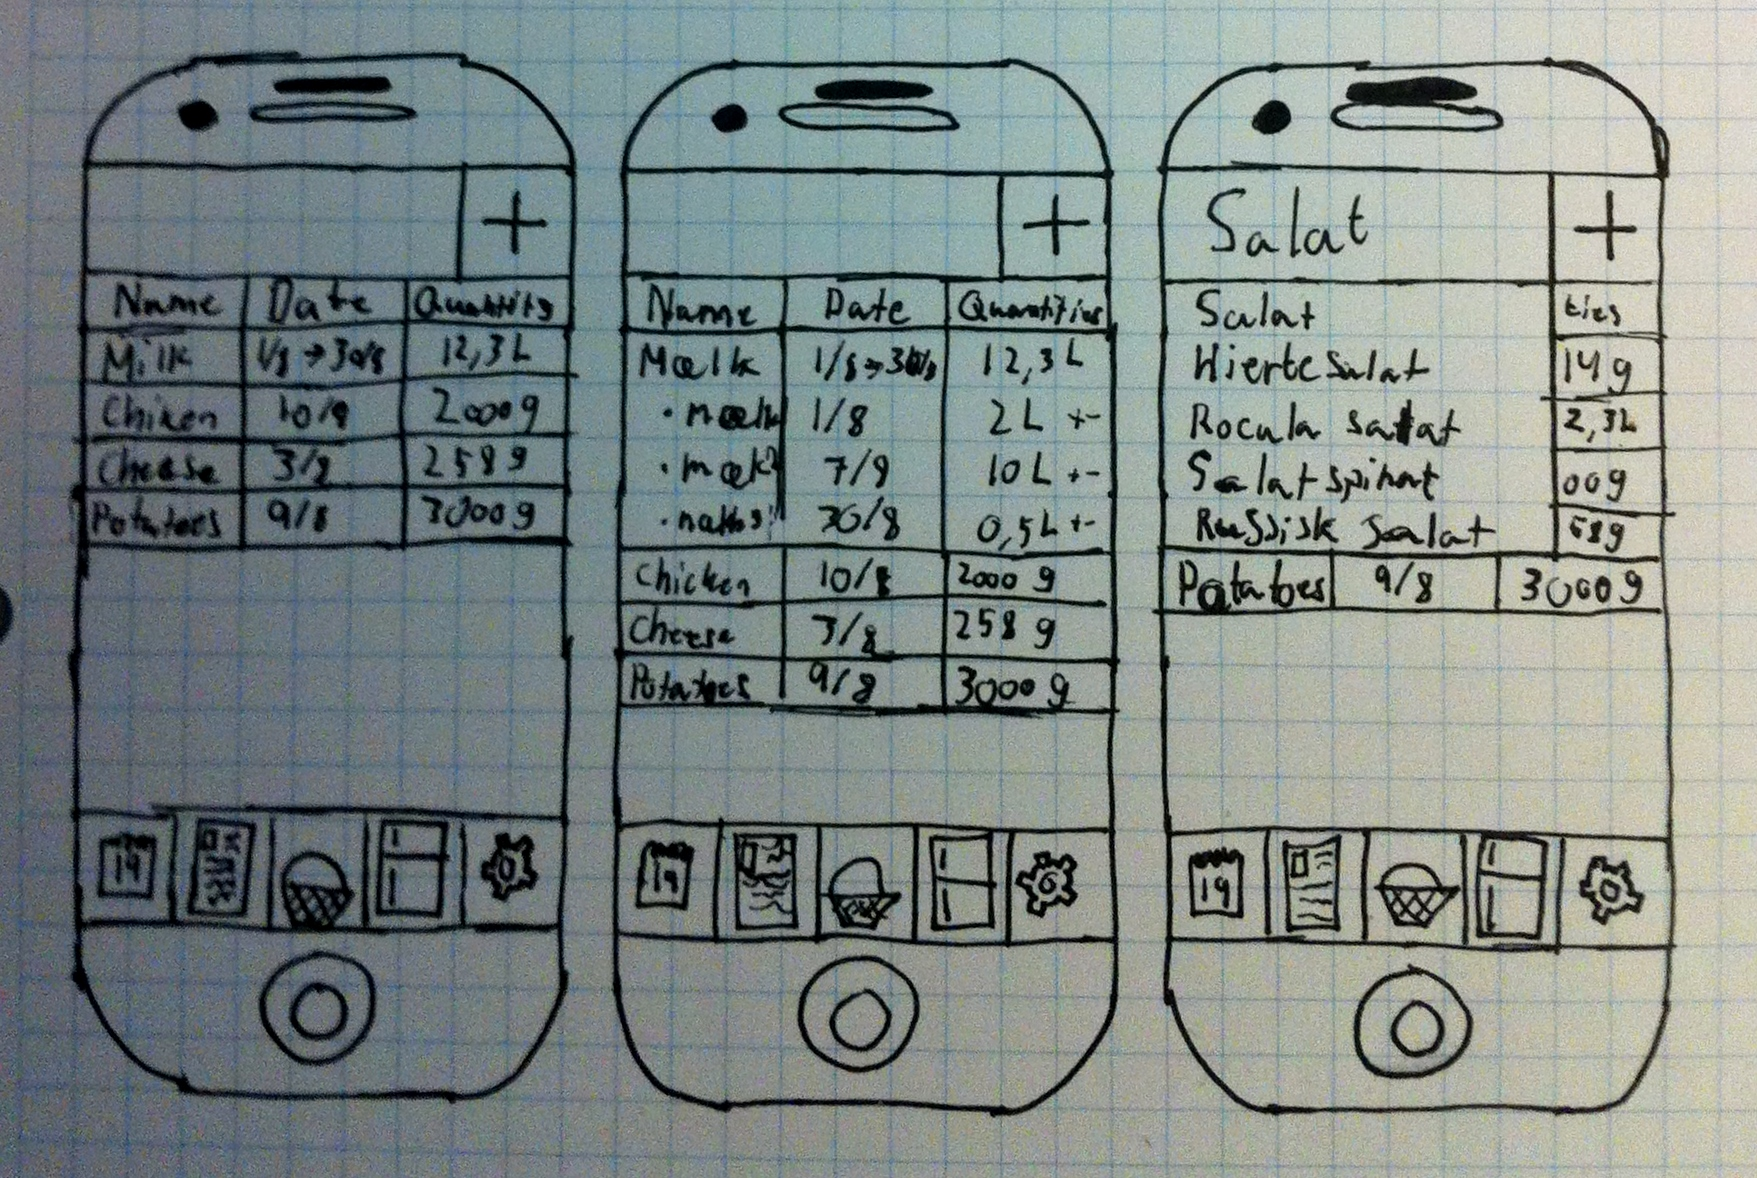
\includegraphics[width=0.5\textwidth]{Grafik/FoodPlanner/FinalInventorySketch}
    \caption{The final sketch of the inventory screens.}
    \label{FinalInventorySketch}
\end{figure}

\textbf{Inventory overview screen:} The inventory overview screen is divided into two different elements, not taking the general design elements into consideration. These elements are:

\begin{itemize}
    \item Search bar
    \item Table
\end{itemize}

The search bar is placed in the top of the screen, as this is where a user most likely will look for it first, because on most mobile applications and also on websites, the search bar is located at the
top of the screen. The add icon enables the user able to add items to the inventory, that are not included in the ingredients of the meal plan.

The second element is the table, which is located under the search bar. The table is divided into three columns; name of the item, expiration date of the item, and the quantity of the item.

The first column shows the name of the items. The second column shows the expiration date of the item. If the user only has one instance of the item, meaning that there will be only one expiration date, only one date is shown in the column, but if the user has multiple instances of an item with different expiration dates, the first and the last expiration date of the item will be shown, separated with an arrow. The quantity column displays the quantity of the item.

\textbf{Expanded ingredient list:}
When the user clicks an ingredient, the ingredient will expand and show all the instances of the information as shown on the second screen from the left in \cref{FinalInventorySketch}. The information is still stored in the three columns described in the inventory overview screen. An instance of the ingredient will therefore show the name of the instance, the expiration date and the quantity of the instance. 

\textbf{Searching for an ingredient:}
The third screen from the left in \cref{FinalInventorySketch} shows the search function of the screen. When text is entered into the search box, the search result items will expand and overlay the ingredients in the inventory.

The new search overlay will show a fixed number of ingredients which contains the searched text in their names. By clicking one of the ingredients, the search results will disappear, and the item chosen will be shown in the search bar. By clicking the add icon the user will now be able to add the item to their inventory, and if the item already is in the inventory, the item will be an instance that the user can expand to see. The expiration date will then be changed in the table, as well with the quantity.